\section{Experimental Results}
\label{sec:experiment}

\subsection{Dataset}
\label{sec:dataset}

\begin{table}
\caption{Statistics of trajectory dataset}
\label{tab:data}
\centering
%\small
%\setlength{\tabcolsep}{3pt} % tweak the space between columns
\begin{tabular}{l*{5}{r}} \hline
\textbf{Dataset} & \textbf{\#Photos} & \textbf{\#Visits} & \textbf{\#Traj.} & \textbf{\#Users} \\ \hline
Edinburgh & 82,060 & 33,944 & 5,028 & 1,454 \\
Glasgow & 29,019 & 11,434 & 2,227 & 601 \\
Melbourne & 94,142 & 23,995 & 5,106 & 1,000 \\
Osaka & 392,420 & 7,747 & 1,115 & 450 \\
Toronto & 157,505 & 39,419 & 6,057 & 1,395 \\
\hline
\end{tabular}
\end{table}


We experiment on five trajectory datasets, namely, Edinburgh, Glasgow, Osaka, Toronto and Melbourne.
The statistics of these trajectory datasets are described in table \ref{tab:data}.
The first four datasets are kindly provided by \cite{ijcai15} and the Melbourne dataset is built using
the same approach introduced by \cite{ht10, ijcai15} which is briefly described below.

Trajectories are extracted using  geo-tagged photos in the Yahoo! Flickr Creative Commons 100M
(a.k.a. YFCC100M) dataset\cite{thomee2016yfcc100m} as well as the Wikipedia web-pages of points-of-interests (POIs).
Photos are mapped to POIs according to their distances calculated by haversine formula\cite{haversine},
and the time that a user arrived a POI is approximated by the time the first photo taken by the user at that POI,
similarly, the time that a user left a POI is approximated by the time the last photo taken 
by the user at that POI. Furthermore, POI visits by a specific user are divided into several pieces according to
the time gap between consecutive POI visits, and the POI visits in each piece are connected in temporal order
to form a trajectory. 
For details of extracting trajectories from geo-tagged photos, please refer to \cite{ht10, ijcai15}.



\subsection{Performance metric}
\label{sec:metric}

\begin{figure}[t]
	\centering
	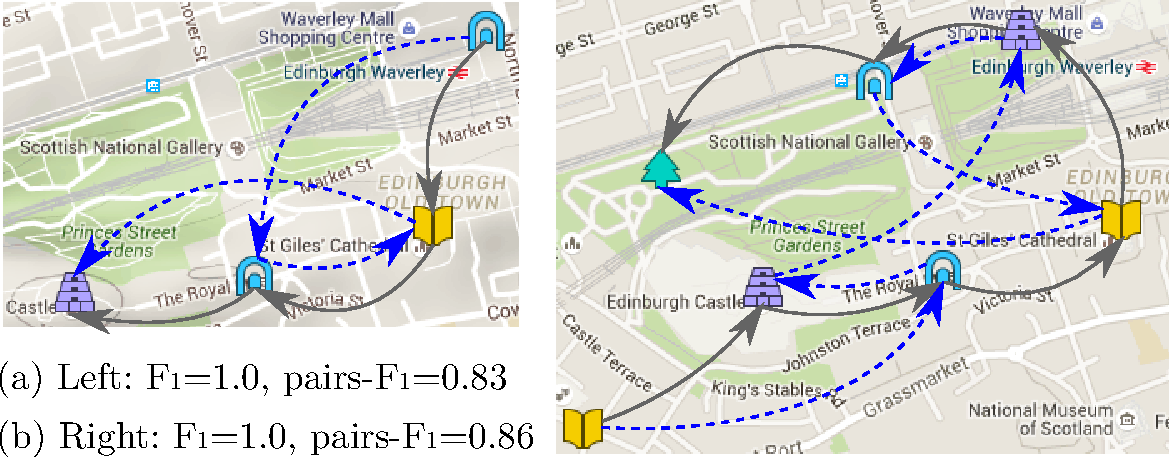
\includegraphics[width=\columnwidth]{fig/pairF1.pdf}
	\caption{$F_1$ vs pairs-$F_1$. Grey: ground truth transitions; dashed blue: recommended transitions. 
    See the third paragraph of Section \ref{sec:metric} for details.}
	\label{fig:pairf1}
\end{figure}


\cheng{Let's try this here. Still needs polishing.}

To evaluate the performance of different trajectory recommendation algorithms,
we employ the trajectory $F_1$-score\cite{ijcai15} to measure the POIs that are
correctly recommended. Let $\mathcal{T}$ be the trajectory that was visited in the real world,
and $\hat{\mathcal{T}}$ be the recommended trajectory,
$\mathcal{P}_{\mathcal{T}}$ be the set of POIs visited in $\mathcal{T}$,
and $\mathcal{P}_{\hat{\mathcal{T}}}$ be the set of POIs visited in $\hat{\mathcal{T}}$,
trajectory $F_1$-score was defined as
\begin{displaymath}
F_1= \frac{2 \times P_{\textsc{point}} \times R_{\textsc{point}}}
          {P_{\textsc{point}} + R_{\textsc{point}}}
\end{displaymath}
where
\begin{displaymath}
P_{\textsc{point}} = \frac{|\mathcal{P}_{\mathcal{T}} \cap \mathcal{P}_{\hat{\mathcal{T}}}|}
                          {|\hat{\mathcal{T}}|},
R_{\textsc{point}} = \frac{|\mathcal{P}_{\mathcal{T}} \cap \mathcal{P}_{\hat{\mathcal{T}}}|}
                          {|\mathcal{T}|}
\end{displaymath}

A perfect trajectory $F_1$-score (i.e., $F_1 = 1$) means the POIs in
the recommended trajectory are exactly the same POIs as those in the ground truth,
and $F_1 = 0$ means that unfortunately none of the POIs in the
real trajectory was recommended.

While trajectory $F_1$-score is good at measure whether POIs are correctly recommended,
it ignores the routes, i.e., the visiting order between POIs.
Two trajectories with the exactly same set of POIs can be completely different to visitors 
given different routes.
Figure \ref{fig:pairf1} illustrates this phenomenon,
the grey lines represent the ground truth transitions that actually visited by tourists
and the dashed blue lines are the recommended trajectory by one of the approaches described
in table \ref{tab:algsummary}.
Even with the exactly same places, the visiting experiences are completely different because 
of dramatically disparate routes.
Enlightened by this observation, we propose a new metric $\text{pairs-}F_1$ that takes into account 
not only the points but also the routes in a trajectory,
\begin{displaymath}
\text{pairs-}F_1 = \frac{2 \times P_{\textsc{pair}} \times R_{\textsc{pair}}}
                       {P_{\textsc{pair}} + R_{\textsc{pair}}}
\end{displaymath}
where
\begin{displaymath}
P_{\textsc{pair}} = \frac{N_c} {|\hat{\mathcal{T}}|(|\hat{\mathcal{T}}|-1) / 2},
R_{\textsc{pair}} = \frac{N_c} {|\mathcal{T}|(|\mathcal{T}|-1) / 2}
\end{displaymath}
and $N_c$ is the number of POI pairs $(p_j, p_k)$ that satisfies the following
constraints\footnote{We define pairs-$F_1=0$ if $N_c$ is $0$.}:
\begin{align*}
    (p_j \prec_{\mathcal{T}} p_k ~\land~ p_j \prec_{\hat{\mathcal{T}}} p_k) & ~\lor~
    (p_j \succ_{\mathcal{T}} p_k ~\land~ p_j \succ_{\hat{\mathcal{T}}} p_k) \\
    p_j \ne p_k, &~~ p_j, p_k \in \mathcal{P}_{\mathcal{T}} \cap \mathcal{P}_{\hat{\mathcal{T}}} \\
    j \ne k, &~~ 1 \le j, k \le |\mathcal{T}|
\end{align*}
where $p_j \prec_{\mathcal{T}} p_k$ denotes POI $p_j$ was visited before POI $p_k$ in trajectory $\mathcal{T}$
and $p_j \succ_{\mathcal{T}} p_k$ denotes $p_j$ was visited after $p_k$ in $\mathcal{T}$.
A perfect pairs-$F_1$, i.e., pairs-$F_1 = 1$, means that both the POIs and their visiting order in the
recommended trajectory are exactly the same as these in the real trajectory,
and pairs-$F_1 = 0$ means that none of the recommended POI pairs was actually visited in the real trajectory.


\subsection{Experimental setup}
\label{sec:setup}

\begin{table*}[t]
\caption{Performance comparison on five datasets in terms of trajectory $F_1$-score.
         The best method for each dataset (i.e., a column) is shown in bold, the second best is shown in italic.}
\label{tab:f1}
\centering
\begin{tabular}{l|ccccc} \hline
 & Edinburgh & Glasgow & Melbourne & Osaka & Toronto \\ \hline
\textsc{Random} & $0.570\pm0.139$ & $0.632\pm0.124$ & $0.558\pm0.149$ & $0.621\pm0.117$ & $0.621\pm0.128$ \\
\textsc{PersTour}\cite{ijcai15} & $0.656\pm0.223$ & $\mathbf{0.802\pm0.213}$ & $0.491\pm0.211$ & $0.702\pm0.230$ & $0.720\pm0.215$ \\
\textsc{PersTour-L} & $0.651\pm0.143$ & $0.660\pm0.102$ & $0.578\pm0.140$ & $0.691\pm0.138$ & $0.642\pm0.112$ \\
\textsc{PoiPopularity} & $\mathbf{0.701\pm0.160}$ & $0.745\pm0.166$ & $0.621\pm0.136$ & $0.661\pm0.128$ & $0.679\pm0.120$ \\
\textsc{PoiRank} & $\mathit{0.694\pm0.157}$ & $\mathit{0.777\pm0.171}$ & $\mathbf{0.626\pm0.137}$ & $0.679\pm0.112$ & $\mathbf{0.748\pm0.166}$ \\
\textsc{Markov} & $0.629\pm0.172$ & $0.714\pm0.168$ & $0.577\pm0.168$ & $0.679\pm0.162$ & $0.663\pm0.157$ \\
\textsc{MarkovPath} & $0.678\pm0.148$ & $0.735\pm0.170$ & $0.596\pm0.147$ & $0.706\pm0.154$ & $0.689\pm0.140$ \\
\textsc{Rank+Markov} & $0.642\pm0.171$ & $0.736\pm0.176$ & $0.598\pm0.169$ & $0.701\pm0.171$ & $0.689\pm0.170$ \\
\textsc{Rank+MarkovPath} & $0.684\pm0.151$ & $0.760\pm0.170$ & $\mathit{0.625\pm0.150}$ & $\mathbf{0.719\pm0.161}$ & $0.724\pm0.152$ \\
\textsc{StructuredSVM} & $0.659\pm0.186$ & $0.727\pm0.173$ & $0.597\pm0.171$ & $\mathit{0.715\pm0.170}$ & $\mathit{0.728\pm0.186}$ \\
\hline
\end{tabular}
\end{table*}


\begin{table*}[t]
\caption{Performance comparison on five datasets in terms of pairs-$F_1$.
         The best method for each dataset (i.e., a column) is shown in bold, the second best is shown in italic.}
\label{tab:pairf1}
\centering
\begin{tabular}{l|ccccc} \hline
 & Edinburgh & Glasgow & Melbourne & Osaka & Toronto \\ \hline
\textsc{Random} & $0.261\pm0.155$ & $0.320\pm0.169$ & $0.249\pm0.148$ & $0.305\pm0.145$ & $0.311\pm0.167$ \\
\textsc{PersTour}\cite{ijcai15} & $0.417\pm0.343$ & $\mathbf{0.646\pm0.366}$ & $0.225\pm0.274$ & $\mathit{0.491\pm0.377}$ & $0.503\pm0.353$ \\
\textsc{PersTour-L} & $0.359\pm0.207$ & $0.352\pm0.162$ & $0.268\pm0.143$ & $0.415\pm0.243$ & $0.331\pm0.159$ \\
\textsc{PoiPopularity} & $\mathit{0.436\pm0.259}$ & $0.509\pm0.299$ & $0.316\pm0.178$ & $0.363\pm0.195$ & $0.385\pm0.202$ \\
\textsc{PoiRank} & $0.424\pm0.249$ & $\mathit{0.565\pm0.312}$ & $0.322\pm0.186$ & $0.376\pm0.173$ & $\mathit{0.512\pm0.295}$ \\
\textsc{Markov} & $0.424\pm0.238$ & $0.488\pm0.283$ & $0.297\pm0.192$ & $0.449\pm0.262$ & $0.419\pm0.237$ \\
\textsc{MarkovPath} & $0.400\pm0.234$ & $0.492\pm0.298$ & $0.294\pm0.187$ & $0.445\pm0.268$ & $0.407\pm0.234$ \\
\textsc{Rank+Markov} & $0.434\pm0.251$ & $0.540\pm0.294$ & $\mathbf{0.357\pm0.210}$ & $0.483\pm0.277$ & $0.462\pm0.266$ \\
\textsc{Rank+MarkovPath} & $0.408\pm0.239$ & $0.532\pm0.304$ & $0.331\pm0.213$ & $0.470\pm0.284$ & $0.465\pm0.266$ \\
\textsc{StructuredSVM} & $\mathbf{0.440\pm0.267}$ & $0.529\pm0.283$ & $\mathit{0.352\pm0.213}$ & $\mathbf{0.508\pm0.292}$ & $\mathbf{0.520\pm0.311}$ \\
\hline
\end{tabular}
\end{table*}


\begin{figure*}[t]
	\centering
	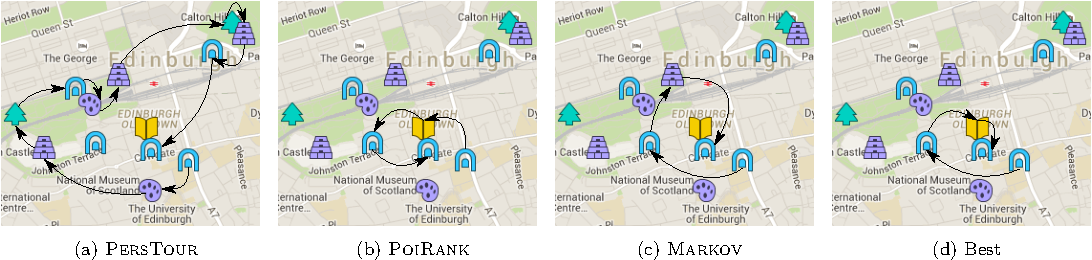
\includegraphics[width=\textwidth]{fig/example-tour.pdf}
	\caption{Different recommendations from algorithm variants. 
    See the main text in Section \ref{sec:casestudy} for description.}
	\label{fig:exampleresult}
\end{figure*}


We use leave-one-out cross validation to evaluate different trajectory recommendation algorithms,
i.e., when testing on a trajectory, all other trajectories are used for training.

% baseline: Random, PersTour, PersTour-L, PoiPopularity
{\bf Baseline approaches} including \textsc{Random} which naively chooses POIs uniformly at random
(without replacement) from the set of POIs $\mathcal{P} \setminus \{p_s, p_e \}$ to form a trajectory.
It does not utilise any features related to POI or query, as shown in  table \ref{tab:algsummary}.
Among the related approaches, \textsc{PersTour}\cite{ijcai15} is the most similar work and it
leverages POI popularity and the sub-tour elimination constraints described in section \ref{sec:walkpath},
the recommended trajectory is also constrained by a time budget.
One variant of \textsc{PersTour} is applying the trajectory length instead of the time budget to constrain
the recommended trajectory, which is denoted as \textsc{PersTour-L} in table \ref{tab:algsummary}.
Another baseline is \textsc{PoiPopularity} described at the beginning of section \ref{sec:method},
it only uses POI popularity to recommend a trajectory as shown in table \ref{tab:algsummary}.

% variants: PoiRank, Markov, MarkovPath, Rank+Markov, Rank+MarkovPath, SSVM
{\bf Variants of point- and route- ranking} approaches including \textsc{PoiRank} 
described in section \ref{sec:ranksvm} that utilises POI and query features, 
and \textsc{Markov} that recommends trajectories uses only transition
probabilities between POIs (section \ref{sec:transition}), 
and its variant \textsc{MarkovPath} that incorporates additional constraints to eliminate sub-tours.
Both \textsc{Rank+Markov} and \textsc{Rank+MarkovPath} described in section \ref{sec:rank+markov}
utilise POI and query features as well as transition probabilities, with the latter uses
additional sub-tour elimination constraints.
Lastly, we have the \textsc{StructuredSVM} that not only utilises POI and query features as well as
transition probabilities but also jointly optimises their relative importance, as described in section \ref{sec:ssvm}.

% Parameters
{\bf Parameters} of these algorithms.
We use a $0.5$ trade-off parameter for \textsc{PersTour} and \textsc{PersTour-L}
and $10.0$ for the regularisation parameter in rankSVM.
The trade-off value in \textsc{Rank+Markov} and \textsc{Rank+MarkovPath} is also $0.5$
and $1.0$ is used as the regularisation parameter in \textsc{StructuredSVM}.


\subsection{Results}
\label{sec:result}


% compare both F1 and pair F1 at the same time
The performance of ten algorithms on five trajectories datasets are shown in table \ref{tab:f1}
and table \ref{tab:pairf1} in terms of trajectory $F_1$-score and pairs-$F_1$ respectively.
%
% 1. all vs Random
% always better than Random, except PersTour on Melbourne which we'll illustrate later
It is obvious that algorithms captured a certain type of information in table \ref{tab:algsummary}
outperforms the \textsc{Random} baseline in terms of both performance metrics on all five datasets,
except the performance of \textsc{PersTour}\cite{ijcai15} on Melbourne dataset which will be interpreted later.

% 2. PersTour vs. PersTour-L
% PersTour always better except on Melbourne which analysed later
\textsc{PersTour}\cite{ijcai15} always performs better than its variant \textsc{PersTour-L},
in particular on Glasgow and Toronto datasets, the advantage gap of \textsc{PersTour}
is significantly large in terms of both performance metrics,
%
% brief mention results of algorithms with and without utilising time budget constraint
which indicate the time budget constraint is more helpful than length constraint for recommending trajectories.
The exception on Melbourne dataset will again explained later.

% go to ranking based algorithms
Despite the utilisation of length constraint, algorithms based on ranking POIs yield very strong performance
by exploring POI and query specific features.
%
% 3. PoiRank vs. PoiPopularity
% PoiRank yields nice improvement on four datasets, only slightly downgraded on Edinburgh
\textsc{PoiPopularity} baseline get pretty good performance despite its simplicity,
and \textsc{PoiRank} yields nice improvements by leveraging more POI features and query specific features,
except slightly worse performance on Edinburgh dataset on which \textsc{PoiPopularity} is the best and
second best performer in terms trajectory $F_1$-score and pairs-$F_1$ respectively.

% go to transition based algorithms
On the other hand, Algorithm that leverage transition probabilities alone does not perform particularly well.
%
% 4. PoiRank vs. Markov:
% in terms of F1, PoiRank always performs much better, except on Osaka where both yield comparable performance
In terms of trajectory $F_1$-score,
\textsc{Markov} can not outperform \textsc{PoiRank} except on Osaka dataset,
on which the performance of both algorithms are comparable.

% in terms of pair F1, PoiRank is significantly better on Glasgow, Melbourne and Toronto, comparable on Edinburgh
In addition, \textsc{PoiRank} performs significantly better than \textsc{Markov} on three datasets, namely,
Glasgow, Melbourne and Toronto.
%
% at the first sight, it seems strange because Markov modelled the transitions and pair F1 measures the visiting order
% but actually pair F1 is affected heavily by the number of correctly predicted POIs, once the POIs are correctly predicted, it will yield
% better pair F1, this is consistent with the observation that, on Osaka dataset, Markov and PoiRank yield comparable F1,
% but Markov outperforms PoiRank significantly in terms of pair F1.
This result may seem strange at first sight because \textsc{Markov} modelled the transition pattern and it would leverage
this advantage to accomplish better performance in terms of pairs-$F_1$ given the fact that this metric is measuring the quality
of visiting order.
However, pairs-$F_1$ is actually affected heavily by the proportion of correctly recommended POIs in trajectory,
once the POIs are correctly predicted, a better pairs-$F_1$ would be achieved,
this supposition can be confirmed by the observation that, on Osaka dataset, \textsc{Markov} and \textsc{PoiRank} achieved
comparable performance in terms of trajectory $F_1$-score, which means the proportion of corrected recommended POIs is comparable,
\textsc{Markov} outperforms \textsc{PoiRank} significantly in terms of pairs-$F_1$,
which suggest the transition information is helpful in some situations.

% 5. PoiRank vs. Markov vs. Rank+Markov
% in terms of both F1 and pair F1,
% when the advantage of PoiRank over Markov is large, Rank+Markov always brings improvements on Markov, but can't compete with PoiRank
% as the advantage gap of PoiRank over Markov shrinks, performance of Rank+Markov becomes closer to PoiRank,
% when the Markov is comparable or better than PoiRank, Rank+Markov outperforms both (Osaka)
% which is consistent with the assumption that transition helps when ranking didn't performs very well
In particular, when the advantage gap of \textsc{PoiRank} over \textsc{Markov} is large,
i.e. Edinburgh, Glasgow, Melbourne and Toronto in table \ref{tab:f1} and Glasgow, Toronto in table \ref{tab:pairf1},
transition information seems not very helpful as \textsc{Rank+Markov}, an algorithm that explores both POI ranking and transitions,
can not compete with \textsc{PoiRank} in both metrics, but nevertheless brings improvements to \textsc{Markov}.
However, as the performance of \textsc{Markov} approaches or surpasses that of \textsc{PoiRank},
i.e., Osaka in table \ref{tab:f1} and Edinburgh, Melbourne, Osaka in table \ref{tab:pairf1},
\textsc{Rank+Markov} outperforms both, this observation indicates that transition information can be very helpful when
ranking does not performs well enough.

% 6. xxPath vs. xx:
% MarkovPath vs Markov:
% in terms of F1, MarkovPath (Rank+MarkovPath) is always better than Markov (Rank+Markov),
% in terms of pair F1, MarkovPath (Rank+MarkovPath) yields comparable or worse performance than Markov.
% which indicates that sub-tour elimination helps POI prediction but worsen the visiting order.
Sub-tour has a non-ignorable effect when recommending trajectories.
We can see from table \ref{tab:f1} that both \textsc{Markov} and \textsc{Rank+Markov} always perform worse,
in terms of trajectory $F_1$-score, than
their counterparts that do not permit sub-tours, namely, \textsc{MarkovPath} and \textsc{Rank+MarkovPath},
which is not unexpected as sub-tours worsen the proportion of corrected
recommended POIs when length constraint is used.
On the contrary, they achieve better performance in terms of pairs-$F_1$ which indicates sub-tours generally
respect the visiting order between POIs.

% go to SSVM
The effect of sub-tours on trajectory recommendation can be further observed through the performance of \textsc{StructuredSVM}.
%
% 7. SSVM vs Rank+Markov and Rank+MarkovPath:
% while SSVM using the same features as Rank+Markov and Rank+MarkovPath, and took advantage of its significantly larger number of parameters
% but SSVM permit sub-tours
% in terms of F1,
% it either yield comparable performance with the better performer (Osaka/Toronto) or with the worse performer (Edinburgh/Glasgow/Melbourne)
% which indicate how hurt sub-tours hurts POI recommendation.
% on the other hand, in terms of pair F1.
% it takes advantage of the transition patterns and yields comparable (Glasgow/Melbourne) or better performance than both of them
While not only utilising the same features as \textsc{Rank+Markov} and \textsc{Rank+MarkovPath},
and but also can further take advantage of the significantly larger number of parameters,
\textsc{StructuredSVM} can only yield comparable performance with the best performer 
among the three at most, when measured in terms of trajectory $F_1$-score.
On the other hand, \textsc{StructuredSVM} makes the best use of transition pattern which leads to comparable or
better performance, in terms of pairs-$F_1$, than both of them all the time.
This observation is consistent with the effect of sub-tours observed above
as \textsc{StructuredSVM} do permit the existence of sub-tours in recommended trajectories.

% 8. PersTour on Melbourne:
% we observed that PersTour was outperformed by Random on Melbourne dataset in terms of both F1 and pair F1.
% it turns out on Melbourne dataset, the many of the ILPs which PersTour solve to get the recommendation result are very hard ILP instances
% in the leave-one-out evaluation, although we utilise a large scale computing cluster with modern hardware,
% there are 12\% of evaluations are failed due to ILP solver can't find a feasible solution in a $2$ hours
% furthermore, a lot recommendations are suboptimal solutions of the ILP due to the $2$ timeout settings.
% which leads to PersTour, which is always a strong performer on other datasets, performs inconsistently on Melbourne dataset.
Lastly, we observed that \textsc{PersTour}, a very good performer in general, is surprisingly outperformed by \textsc{Random} baseline
on Melbourne dataset in terms of both trajectory $F_1$-score and pairs-$F_1$.
It turns out that, on this very dataset, many of the integer linear programming (ILP) problems
which \textsc{PersTour} need to solve to get the recommendation results are hard ILP instances.
In the leave-one-out evaluation, although we utilised a large scale computing cluster with modern hardware,
there are still $12\%$ of evaluations failed due to the ILP solver can not find a feasible solution in $2$ hours.
Furthermore, a lot of recommendations are produced from suboptimal solutions of the corresponding ILPs due to
the $2$ hours timeout setting, these results lead to the generally strong performer \textsc{PerTour} performs
inconsistently on Melbourne dataset.


\subsection{Case study}
\label{sec:casestudy}


Figure \ref{fig:exampleresult} illustrates a test case in Edinburgh dataset.
The ground truth is a trajectory of length $4$ that starts at a POI of category \textit{Structures},
visits two intermediate POIs of category \textit{Structures} and \textit{Cultural} and 
terminates on a POI of category \textit{Structural}.

The trajectory recommended by \textsc{PersTour} is a tour with $11$ POIs, as shown in figure \ref{fig:exampleresult}(a),
with none of the intermediate POIs visited.
\textsc{PoiRank} (figure \ref{fig:exampleresult}(b)) recommended a tour with correct POIs, but the routes are completely wrong.
On the other hand, \textsc{Markov} (figure \ref{fig:exampleresult}(c)) missed one POI but the recommended route for one of 
the intermediate is consistent with the ground truth.

The best recommendation, as shown in figure \ref{fig:exampleresult}(d), with exactly the same points and routes as the ground truth,
which in this case is achieved by \textsc{Rank+MarkovPath}.



% Figures from the appendix
\begin{figure*}[t]
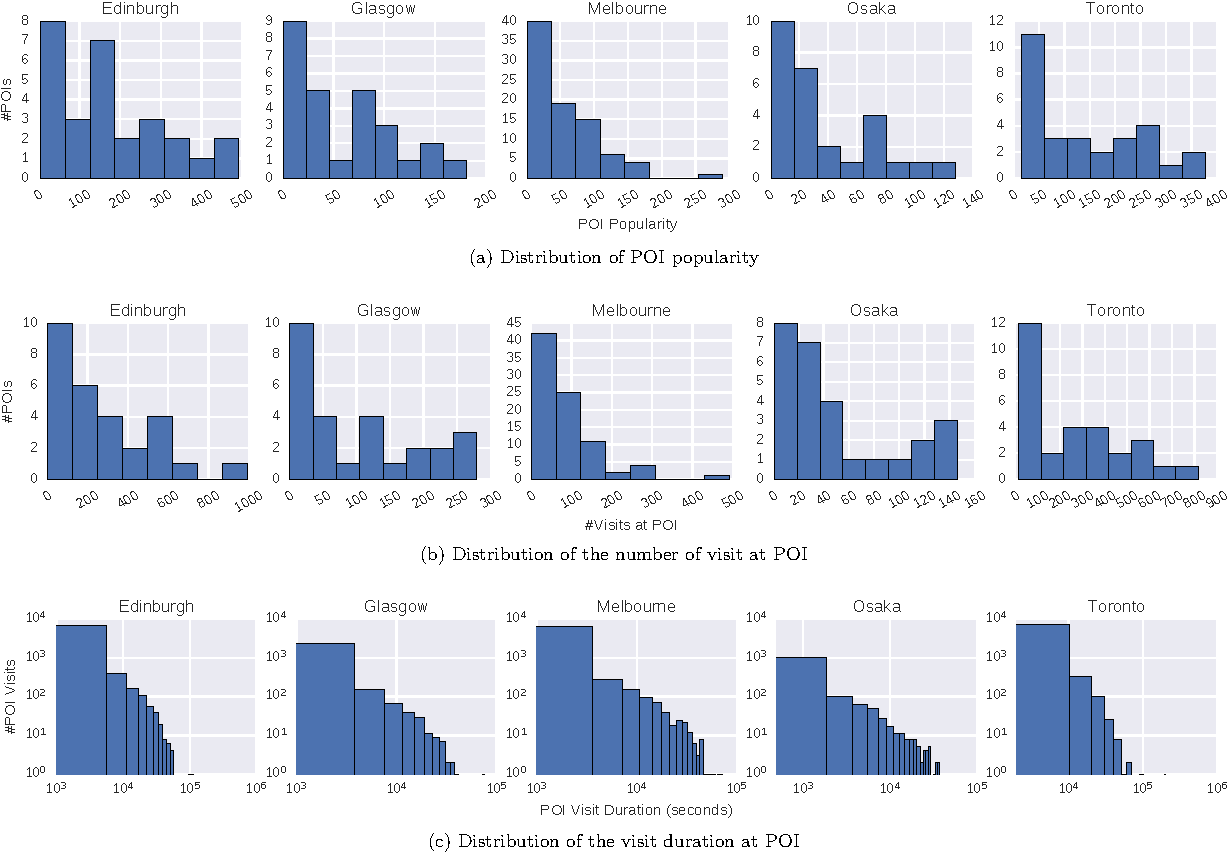
\includegraphics[width=\textwidth]{fig/feature_distro.pdf}
\caption{Distribution of POI popularity, the number of visit and visit duration}
\label{fig:distro}
\end{figure*}
